% Chapter 2
\chapter{Chapitre 2 : Intelligence en essaim : BSO, EHO, ESWSA et GA} % Main chapter title

\label{Chapter2} % For referencing the chapter elsewhere, use \ref{Chapter1} 

%----------------------------------------------------------------------------------------


\vspace{-0.5cm}
\section{Introduction}
Dans ce chapitre nous allons présenter les outils intelligents de résolution pour notre problématique. Ces derniers consistent en des méta-heuristiques inspirées de l'intelligence collective des animaux et insectes, autrement dit l’intelligence en essaim.

Nous commencerons par introduire les algorithmes basés intelligence en essaim et leurs principaux paramètres, suivis d'un décryptage des trois approches choisies pour notre étude, à savoir :
\begin{itemize}
	
	\item Bee Swarm Optimization (BSO) qui est un algorithme de résolution s'inspirant de l'intelligence collective du comportement des abeilles lors de la recherche de nourriture. BSO a fait ses preuves face à de nombreux problèmes d'optimisation combinatoire (le problème de satisfiabilité SAT, le problème du voyageur de commerce, ...etc.).
	
	\item Elephant Herding Optimisation (EHO) et Elephant Swarm Water Search Algorithm (ESWSA), tous deux des algorithmes inspirés du comportement des éléphants en groupe.
	
	\item On verra aussi l'algorithme génétique (GA) dans sa version GA incrémental.
\end{itemize}

On clôturera ce chapitre par les motivations qui nous ont poussées à choisir ces algorithmes intelligents comme méthodes de résolution pour la détection de cibles.


\section{Les algorithmes basées intelligence en essaim}
Swarm Intelligence ou l’intelligence en essaim étudie le comportement coopératif entre les espèces naturelles. C’est un domaine prometteur de l'intelligence artificielle dont le principe de base repose sur l'observation par la nature des phénomènes intelligents et surtout des comportements de groupe chez les animaux.

Une approche ou méthode basée intelligence en essaim est également considérée comme une méta-heuristique. Elle suit un schéma d'algorithme évolutif, dicté par la simulation de l'évolution des espèces naturelles \cite{courshabiba}.
\\

Les méta-heuristiques sont des approches génériques qui visent à proposer des solutions à des problèmes complexes, en employant une certaine stratégie d'exploration de l'espace de recherche appelée \textbf{espace des solutions}. Ce dernier comporte toutes les solutions possibles au problème. Ces \textbf{solutions} sont ensuite filtrées grâce à une \textbf{fonction objectif} permettant de les ordonner selon leur optimalité \cite{courshabiba}.\\

La figure \ref{metas} montre qu’il existe deux catégories principales de méta-heuristiques. Les méta-heuristiques basées sur une solution unique, telles que, la recherche tabou (TS)  \cite{aouatTS}, recuit simulé, la recherche locale guidée (GLS) \cite{habibaGLS}, ...etc, et les méta-heuristiques basées population comme l'algorithme génétique (GA) \cite{kechidGA} ou une de ses extensions, Les algorithmes mémétiques  (MA) \cite{habibaMA}, la recherche par dispersion (SS) \cite{habibaSS-GA}, l'algorithme Bat (BA) \cite{boukraBA-ACO,habibaBA2}, les colonies de fourmis (ACS)  \cite{habibaACO}, l'algorithme d'optimisation par essaim de particules (PSO) \cite{habibaPSO}, l'algorithme des lucioles FFA (Firefly algorithm) \cite{habibaFAA}, l'essaim d'abeilles à savoir BSO (Bee Swarm Optimization) \cite{habibaBSO1,kechidBSO}, ABSO (Advenced Bee Swarm Optimization) \cite{habibaABSO}, ou encore ABC (Artificial Bee Colony) \cite{boukraABC} etc.

Les algorithmes basés intelligence en essaim peuvent être vus comme des méta-heuristiques basées population \cite{courshabiba}.

Ces nombreux travaux ont été développés au sein du laboratoire de recherche en l'intelligence artificielle LRIA \footnote{https://www.lria.usthb.dz/}.

\noindent
\begin{center}	  
	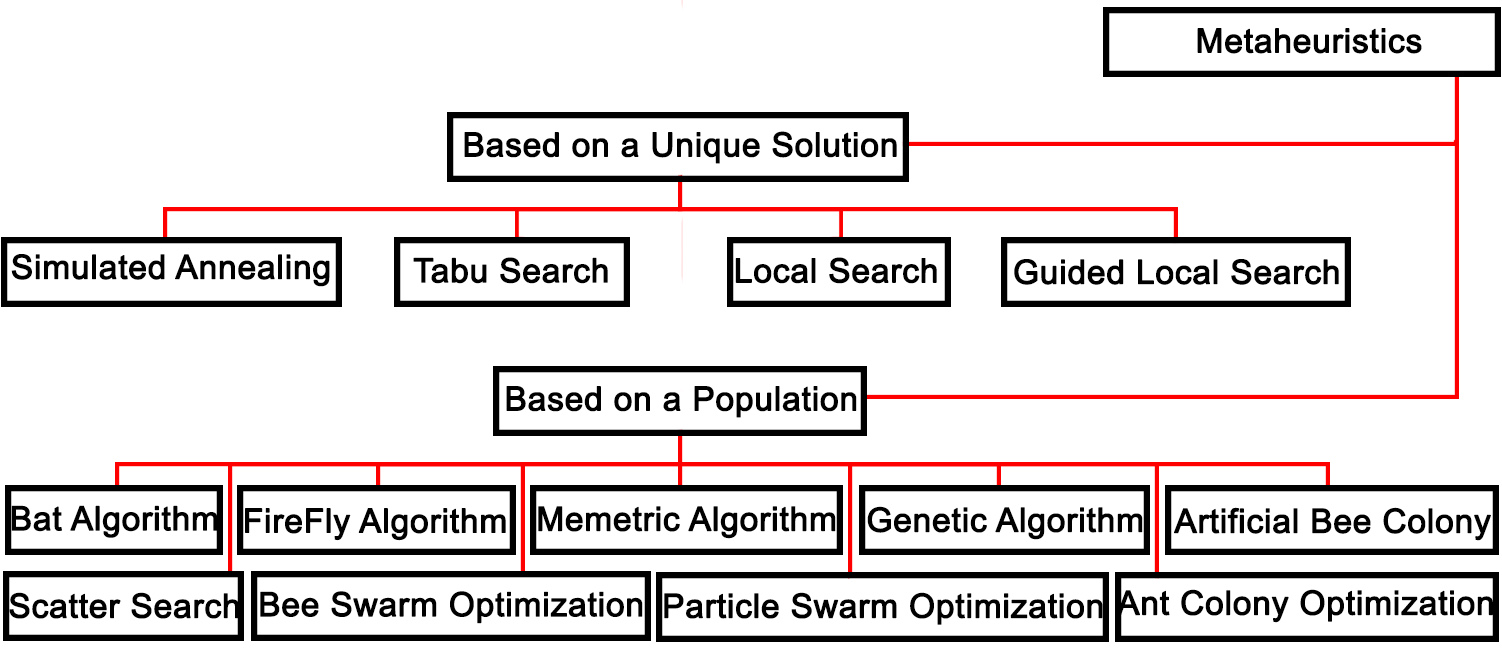
\includegraphics[width=0.9\textwidth]{metagraph.jpg}%
	\vspace{-0.1 cm}
	\captionof{figure}{Classification des méta-heuritiques}\label{metas}%
\end{center}


Étant donné l'efficacité et la simplicité des méta-heuristiques, on va s'intéresser de plus près à BSO, EHO, ESWSA et GA qui sont des méta-heuristiques basées population ayant connu un large intérêt et succès.

\section{Bee Swarm Optimization \cite{Drias}}

\subsection{Inspiration des abeilles}
De nombreuses études biologiques se sont intéressées aux comportements et à la psychologie des abeilles afin de décortiquer leurs méthodologies et stratégies de recherche du nectar ainsi que leur façon de communiquer les informations concernant leurs trouvailles.

L'une des expériences les plus connues sur les abeilles, est celle de Seeley, Camazine et Sneyd en 1991 \cite{Seeley}, elle a abouti sur les quelques caractéristiques suivantes :
\\

\begin{itemize}
	
	\item[$\bullet$] la catégorie d'abeilles \textit{"travailleuses"} est celle qui se charge de trouver la nourriture ("Scout bee"). Les abeilles reviennent à la ruche en ramenant un peu de leurs récoltes.
	
	\item[$\bullet$]Les abeilles ont tendance à privilégier les régions qui regorgent de nourriture aussi lointaines soient elles aux zones moins riches en pollen, mais à proximité de la ruche.
	
	\item[$\bullet$] L'abeille ayant trouvé la meilleure région en termes de nourriture effectuera la danse la plus rigoureuse, ce qui guidera l'essaim vers la meilleure région.
	
	\item[$\bullet$] La danse (mouvement circulaire) est le moyen de communication entre les abeilles, elle englobe les informations concernant la quantité, la direction et la distance entre la ruche et la région où se trouve la nourriture.
\end{itemize}

\subsection{Analogie entre le comportement des abeilles et BSO}
BSO est entièrement inspirée du comportement des abeilles pour la recherche du pollen, ci-dessous le tableau \ref{analogieBSO} fait l'analogie entre le comportement des abeilles travailleuses et leurs représentations simplifiées dans BSO :\\

\begin{table}[h]
	\centering
	\begin{tabular}{|p{7cm}|p{7cm}|} 
		\hline
		
		\textbf{Essaim d'abeilles} & \textbf{BSO}\\ 
		
		\hline
		Une abeille éclaireuse est envoyée dans un champ de fleurs et se positionne sur une fleur aléatoirement. &  
		Une solution est générée aléatoirement à partir de l'espace des solutions, elle est ensuite affectée à l'abeille de référence. \\ 
		\hline
		Les abeilles s'orientent vers les champs de fleurs à la recherche de quantité de nourriture (pollen). & Les abeilles artificielles se déplacent dans l'espace des solutions à la recherche de bonnes solutions.\\
		\hline
		Les abeilles se dispersent autour de la zone indiquée par l'abeille éclaireuse pour couvrir au mieux le champ de fleurs. &  La diversification est basée sur le Flip. Ce dernier permet la génération d'un certain nombre de solutions à partir de la solution de référence. \\ 
		\hline
		%			\end{tabular}
		%\end{table}
		%\begin{table}[h]
		%	\centering
		%	\begin{tabular}{|p{7cm}|p{7cm}|} 
		%		\hline	
		Chaque abeille procède à une recherche locale dans sa zone d'atterrissage. & 
		Chaque abeille porteuse d'une solution effectue une recherche locale, ce processus est appelé \textit{"intensification"}.  \\
		\hline
		Chaque zone de fleurs est évaluée selon la quantité de pollen qui s'y trouve. &  Chaque solution est évaluée selon la fonction objectif.\\ 
		\hline
		Chaque abeille se rappelle de la fleur source ayant la plus grande quantité de pollen ainsi que l'endroit où elle se trouve. Elle se met à danser juste au-dessus pour en informer l'essaim. &  Chaque abeille sauvegarde sa meilleure solution locale dans une table appelée \textit{Table Dance}.\\ 
		\hline
		La vigueur de la danse de l'abeille est proportionnelle à la richesse et quantité de nourriture trouvée.
		& 	La sélection d'une solution de la table \textit{Dance} se base sur un critère de qualité. Toutes les abeilles sont mises au courant de la meilleure solution actuelle. \\
		\hline
		En cas de recherche non-fructueuse, les abeilles explorent d'autres zones distantes & en cas de stagnation de la recherche, la solution la plus diverse de la table \textit{Dance} est sélectionnée comme solution de référence. \\ 
		\hline
		%\bottomrule
	\end{tabular}
	\captionsetup{width=1\linewidth}
	\caption{Analogie entre les caractéristiques des essaims d'abeilles et BSO.}
	\label{analogieBSO}
\end{table}

\newpage

\subsection{Paramètres et fonctions}
BSO est caractérisée par plusieurs paramètres empiriques, qui sont : 
\begin{itemize}
	\item[$\bullet$] \textbf{nbrBee} : le nombre d'abeilles de l'essaim.
	\item[$\bullet$] \textbf{Flip} : la fréquence d'inversement.
	\item[$\bullet$] \textbf{MaxChance} : le nombre de chances maximal. 
	\item[$\bullet$] \textbf{MaxItération} : le nombre d'itérations maximal.\\
\end{itemize}

\textbf{Sref:} La solution de référence est initialisée aléatoirement au début de la recherche, puis mise à jour selon les étapes de BSO, par la meilleure solution en termes de qualité ou de diversité.\\ 

\textbf{Flip:}
C'est un paramètre qui détermine le nombre de variables à inverser au niveau de la solution de référence (Sref) afin d'obtenir de nouvelles solutions. $\frac{n}{flip}$ représente ainsi la distance qui sépare les nouvelles solutions de \textit{Sref}, \textit{n} étant la taille de la solution. \\

\textbf{Détermination des zones de recherche:}
l'application du \textit{Flip} sur une solution de référence génère un ensemble de solutions équidistantes de \textit{Sref}, formant un cercle autour d'elle.\\


\textbf{Recherche locale:}
Chaque abeille effectue une recherche locale à partir de la solution qui lui est affectée afin d’évaluer les solutions voisines en ne gardant que la meilleure.\\

\textbf{MaxChance:}
Chaque solution possède un nombre de chances maximal pour être choisie comme solution de référence à chaque itération.\\


\textbf{Table dance:}
La table \textit{"Dance"} est le répertoire commun à toutes les abeilles de l'essaim pour y inscrire leurs meilleures solutions locales.\\

\subsection{Pseudo-code BSO}
\vspace{-0.2cm}
\begin{algorithm}[H]
	\TitleOfAlgo{BSO}
	\vspace{-0.2cm}	
	\xdash[13.5cm]
	
	\SetAlgoLined
	\DontPrintSemicolon
	\KwIn{$MaxIteration,Flip,Maxchances,Optimale,nombre d'abeilles$}
	\KwOut{$meilleureSolution$ : la meilleure solution trouvée}
	
	\SetKwFunction{solutionAleatoire}{solutionAléatoire()}
	\SetKwFunction{Insertion}{Insertion}
	\SetKwFunction{DeterminationDesZonesDeRecherche}{DeterminationDesZonesDeRecherche}
	\SetKwFunction{rechercheLocale}{rechercheLocale}
	\SetKwFunction{MeilleureDeDance}{MeilleureDeDance}
	
	\tcc{génération aléatoire de la solution de reference.}
	$Sref \gets$ \solutionAleatoire\;
	$meilleureSolution \gets Sref$\;
	
	\tcc{Tant que le nombre d'itérations maximal n'est pas atteint et la solution optimale n'est pas trouvée réitérer}
	\While{$\neg$  ($MaxIteration$ \textbf{or} $Optimale$) }{
		\tcc{Insertion de la solution de référence dans la liste Tabou}
		\textbf{\Insertion($listeTabou$,$Sref$)}\;
		\tcc{Affectation des zones de recherche aux abeilles}
		$abeilles \gets$
		\DeterminationDesZonesDeRecherche($Sref$)\;
		
		\ForEach{$abeille \in abeilles$}
		{
			\tcc{Effectuation d'une recherche locale}
			$solutionLocale \gets$ \rechercheLocale($abeille$)\;
			\tcc{Evaluation et insertion de la meilleure solution locale dans la table Dance.}
			\Insertion($Dance$,$MeilleuresolutionLocale$)\;
		}
		\tcc{Sélection de la meilleure solution de la table Dance.}
		$Sref \gets $\MeilleureDeDance($Dance$)\;
		\If{$sRef > meilleure$ }{
			\tcc{Sauvgarde de la nouvelle meilleure solution.}
			$meilleureSolution \gets sRef$\;
		}
	}
	\Return $meilleureSolution$\;
	\caption{BSO Générique}
\end{algorithm}

\textbf{ }


\begin{function}[H]
	\TitleOfAlgo{DéterminationDesZonesDeRecherche}
	\vspace{-0.2cm}		
	\xdash[13.5cm]
	
	\SetAlgoLined
	\DontPrintSemicolon
	\KwIn{$Flip$ : fréquence d'inversement}
	\KwOut{$ensemble\_K\_solutions$ : ensemble de K solutions}
	$h \gets 0$\;
	
	\SetKwFunction{Inverser}{Inverser}
	
	
	\While{$taille(espace_{recherche}) < k$ \textbf{and} $h < Flip $}
	{ $s \gets Sref$; 	$p \gets 0$\;
		\tcc{Inversion partielle de la solution, à une fréquence : flip}
		\Repeat{$Flip*p+h>n$}
		{
			
			$s \gets$ \Inverser($s,s[Flip*p+h]$)\;
			$p \gets p + 1$\;
			
		}
		\tcc{Insertion de la solution générée dans la liste de solutions}
		$ensemble\_K\_solutions \gets ensemble\_K\_solution\cup$ $\{s\}$\;
		$h \gets h + 1$\;
	}
	
	\Return $ensemble\_K\_solutions$\;
	
	\caption{DéterminationDesZonesDeRecherche()}
	
\end{function}






%\newpage

\section{EHO \& ESWSA : Deux algorithmes basés essaim d'éléphants}
\subsection{Inspiration des éléphants}
Les éléphants sont des mammifères sociaux qui présentent des structures sociales complexes ayant une multitude de particularités surprenantes.


Dans un premier temps, on se contentera d'exhiber les caractéristiques individuelles suivantes \cite{EHO1} :


\begin{itemize}
	
	\item[$\bullet$] Bonne mémoire.
	\item[$\bullet$] Font preuve d'une intelligence avancée (reconnaissance de soi, la conscience de soi).
	\item[$\bullet$] Capacité d'apprendre et de distinguer plusieurs discriminations visuelles et acoustiques.
	\item[$\bullet$] Capacité à utiliser et manipuler des outils de la vie réelle.
	\item[$\bullet$] Possession de systèmes de détection et de communication très avancés.
\end{itemize}
\textbf{ }\\
\textbf{ }
Quant aux caractéristiques de groupe, nous citons \cite{EHO2} :


\begin{itemize}
	\item[$\bullet$] Un groupe d'éléphants est composé de plusieurs clans.
	\item[$\bullet$] Un clan est dirigé par une matriarche (souvent l'éléphant le plus vieux du troupeau).
	\item[$\bullet$] Les femelles préfèrent vivre dans des groupes familiaux (clan).
	\item[$\bullet$] Les éléphants mâles ont tendance à quitter leur groupe familial en grandissant.
	\item[$\bullet$] Les éléphants mâles loin de leur groupe familial peuvent rester en contact avec les éléphants de leur clan par le biais de vibrations basses fréquences.
	
\end{itemize}

%~\cite{ref1} \cite{ref2}

\subsubsection*{Méthodes de communication \cite{EHO1}:}

Les éléphants utilisent leurs sens de l'ouïe, de l'odorat, de la vision, du toucher et une capacité exceptionnelle à détecter les vibrations pour communiquer entre eux ainsi qu'avec les autres espèces. Il existe deux types courants de communication entre éléphants:

\begin{enumerate}
	\item \textbf{Communication à longue distance:} (jusqu'à 10-12 km)\\
	\textit{-Les communications sismiques}, causées par le grondement et le mouvement des éléphants. Leur réception se fait à travers leurs mécano-récepteurs dans les orteils ou les pieds et la pointe de leurs trompes.\\
	\vspace{-0.2cm}
	
	\textit{-Les communications sonores} produisent une gamme de signaux sonores (infrasons) que leurs trompes peuvent amplifier. Leurs oreilles font office de parabole pour la réception des sons de basses fréquences d'autres éléphants lointains. \\
	\vspace{-0.2cm}
	
	\textit{-Les communications chimiques (olfactives)},  ils utilisent leurs trompes pour sentir l'air, ou pour explorer le sol et les arbres, ainsi que pour renifler d'autres éléphants. 
	
	\item \textbf{Communication à courte distance:}\\
	\textit{-Les communications visuelles,} la vision des éléphants atteint une portée maximale de 46-100 m. Ils utilisent la tête, les yeux, la bouche, les oreilles, la trompe et tout le corps pour l'échange de messages.\\
	\vspace{-0.2cm}
	
	\textit{-Les communications tactiles}, les éléphants sont des animaux extrêmement tactiles. Ils communiquent par le toucher en utilisant leurs trompes, leurs défenses, leurs pieds, leurs queues, ...etc.
	
\end{enumerate} 

\subsection{EHO : Elephant Herding Optimization}
\subsubsection{Analogie entre les éléphants et EHO \cite{EHO2}}

La méta-heuristique \textbf{EHO} simule l'évolution du mouvement des éléphants. Elle représente un comportement simplifié des groupes d'éléphants se basant sur les règles idéalisées présentées dans le tableau qui suit :

\begin{table}[h]
	\centering
	\begin{tabular}{|p{7cm}|p{7cm}|} 
		\hline
		
		\textbf{Clans d'éléphants} & \textbf{EHO}\\ 
		\hline
		Les éléphants parcourent la nature à la recherche de meilleures sources de nourriture et d'eau
		&  Les éléphants artificiels se déplacent dans l'espace des solutions cherchant la meilleure solution globale au problème à traiter.\\
		\hline
		La quantité de nourriture et d'eau permet aux éléphants d'évaluer la qualité de l'environnement 
		&  La qualité de la solution est évaluée à travers la fonction objectif.\\
		\hline
		Les éléphants vivent en clans où chaque clan est composé de plusieurs éléphants. &  
		Plusieurs clans (\textbf{nClan}) sont créés avec un nombre fixe d'éléphants \textbf{N}, une solution est affectée à chaque éléphant. \\ 
		\hline
		Les éléphants de chaque clan vivent sous la direction d'une \textit{matriarche} qui guide leurs déplacements. & 
		L'éléphant possédant la meilleure solution du clan (meilleure locale) guide le clan.\\
		\hline
		Un nombre déterminé d'éléphants mâles quittera leur groupe familial et vivra solitairement loin du groupe d'éléphants principal à chaque génération. &  Le pire éléphant en termes d'évaluation, devra se détacher de son clan et explorer une nouvelle zone à chaque itération. \\ 
		\hline
		%\bottomrule
	\end{tabular}
	\captionsetup{width=1\linewidth}
	\caption{Analogie entre les caractéristiques des éléphants et EHO.}
	\label{analogieEHO}
\end{table}


\vspace{-0.5cm}


\subsubsection{Paramètres et fonctions \cite{EHO2}}

Cette méthode repose sur un certain nombre de paramètres empiriques, qui sont : 
\begin{itemize}
	\item[$\bullet$] \textbf{nClan} : le nombre de clans.
	\item[$\bullet$] \textbf{N} : le nombre d'éléphants d'un clan.
	\item[$\bullet$] \textbf{$\alpha$} : le taux d'influence de la matriarche sur un éléphant. 
	\item[$\bullet$] \textbf{$\beta$} : le taux d'influence du centre de gravité du clan sur la matriarche.
\end{itemize}

Pour le calcul des positions futures des éléphants et de la dynamique des clans, l'algorithme est basé sur trois fonctions principales, soient :

\begin{itemize}
	\item[$\bullet$] Pour chaque éléphant \textbf{i} du clan \textbf{c}, sa prochaine position est calculée par l'équation suivante :
	\begin{equation}
	\label{eq:xnew}
	{X}_{new,c, i} = {X}_{c, i}  +  \alpha *( {X}_{Best,c}- {X}_{c, i} ) * r 
	\end{equation}
	Avec:
	$r \in $[0, 1] : distribution uniforme.\\
	${X}_{c, i}$ et ${X}_{new,c, i}$ : positions (avant et après) du $i^{\grave{e}me}$ éléphant dans le clan c.\\ 
	$\alpha \in $[0,1] : taux d'influence de la matriarche sur le $i^{\grave{e}me}$ éléphant.\\
	
	\item[$\bullet$] Pour l'éléphant matriarche du clan \textbf{c}, sa position future est calculée comme suit:
	\begin{equation}
	\label{eq:xbest}
	{X}_{Best,c}  =  \beta  *  {X}_{center,c} 
	\end{equation}
	Avec: 
	${X}_{center,c}$ : le centre de gravité du clan c.\\
	$\beta$ : le taux d'influence du centre de gravité du clan sur la matriarche.\\
	
	Sachant que le centre de gravité est donné par la formule suivante:
	\begin{equation}
	\label{eq:xcenter}
	{X}_{center,c}  = \frac{1}{N} * \sum_{i=1}^{N} {X}_{c,i}
	\end{equation}
	
	\item[$\bullet$] Pour le pire éléphant (\textit{Worst}) qui quittera le clan, sa position est déterminée par l'estimation:
	\begin{equation}
	\label{eq:xworst}
	{X}_{Worst,c}  =  {X}_{min} + ({X}_{max} - {X}_{min}) * rand
	\end{equation}
	Avec:
	$rand \in $ [0, 1]  : distribution stochastique uniforme.\\
	${X}_{min}$ et ${X}_{max}$ : limites (inférieure, supérieure) de la position d'un éléphant.
\end{itemize}


\subsubsection{Pseudo code de EHO \cite{EHO2}}
\begin{algorithm}[H] 
	\TitleOfAlgo{EHO}
	\vspace{-0.2cm}	
	\xdash[13.5cm]
	
	\SetAlgoLined
	\DontPrintSemicolon
	\KwIn{MaxGen : le nombre maximum de générations, }
	\KwOut{meilleure solution}
	
	\SetKwData{MaxGen}{MaxGen}
	\SetKwData{t}{t}
	\SetKwFunction{ClanUpdatingPosition}{MAJPositionClan}
	\SetKwFunction{SeparatingOperator}{OperateurSéparation}
	\SetKwFunction{EvaluatePopulation}{EvaluationPopulation}
	\SetKwFunction{SortElephant}{TriElephant}
	\SetKwFunction{initPopulation}{initPopulation}
	\SetKw{rt}{Retourner}
	
	
	\Begin
	{
		\textbf{Initialisation}\\
		
		\t=1;	\tcc{Initialisation du compteur de générations}
		
		\initPopulation();\tcc{initialisation des solutions des éléphants.}
		
		\While{ \t $<$ \MaxGen}
		{	
			\tcc{Tri de tous les éléphants selon la fonction d'évaluation.}
			\SortElephant();\\
			%\vspace{0.3cm}
			
			\tcc{Mise à jour de la position des éléphants de chaque clan.}
			\ClanUpdatingPosition();\\
			%\vspace{0.3cm}
			
			\tcc{Mise à jour de la position du pire éléphant de chaque clan.}
			\SeparatingOperator();\\
			%\vspace{0.3cm}
			
			\tcc{Évaluation de la population.}
			\EvaluatePopulation(); 
			
			\t $\gets$ \t + 1;
		}
	}
	\caption{\textbf{EHO Générique}}
\end{algorithm}

\textbf{ }

\begin{function}[H]	
	\TitleOfAlgo{MAJPositionClan}
	\vspace{-0.2cm}		
	\xdash[13.5cm]
	
	\SetAlgoLined
	\DontPrintSemicolon
	\KwIn{$nClan$ : nombre de clans, 
		$N$ : nombre d'éléphants d'un clan }
	%	\KwOut{}
	
	\SetKwData{i}{i}
	\SetKwData{c}{c}
	\SetKwData{nClan}{nClan}
	
	\tcc{pour chaque clan de la population}
	\For{ \c $\gets$ 1 \KwTo \nClan}
	{
		\vspace{0.1cm}
		\tcc{pour chaque éléphant du clan c}
		\For{\i $\gets$ 1 \KwTo N}
		{
			Mise à jour de $X_{c,i}$ et calcul de $X_{new,c,i}$ selon Eq. ($\ref{eq:xnew}$).\\
			\vspace{0.1cm}
			\If{ $X_{c,i} =X_{Best,c}$}
			{
				Mise à jour de $X_{c,i}$ et calcul de $X_{new,c,i}$ selon Eq. ($\ref{eq:xbest}$).
			}
		}			
	}
	
	\caption{MAJPositionClan()}
\end{function}
\vspace{0.1cm}
\begin{function}[H]
	\TitleOfAlgo{OpérationSéparation}
	\vspace{-0.2cm}		
	\xdash[13.5cm]
	
	\SetAlgoLined
	\DontPrintSemicolon
	\KwIn{nClan : nombre de clan de la population}
	
	\SetKwData{c}{c}
	\SetKwData{nClan}{nClan}
	
	\tcc{pour chaque clan de la population}
	\For{ \c $\gets$ 1 \KwTo \nClan}
	{
		Remplacer le pire éléphant du clan $c$ selon Eq. ($\ref{eq:xworst}$).
	}
	\caption{OpérationSéparation()}
\end{function}












\subsection{ESWSA : Elephant Swarm Water Search Algorithm}
\subsubsection{Analogie entre les éléphants et ESWSA \cite{EHO1}}
L'algorithme évolutionnaire ESWSA proposé par \textit{S Mandal}, simule aussi l'évolution du
mouvement des éléphants mais pour la recherche d'eau. La métaphore entre le milieu
naturel et la résolution de problèmes est présentée dans le tableau \ref{analogieESWSA} suivant :


\begin{table}[h]
	\centering
	\begin{tabular}{|p{7.5cm}|p{7.5cm}|} 
		\hline
		
		\textbf{Groupes d'éléphants} & \textbf{ESWSA}\\ 
		\hline
		Les éléphants sont à la recherche de meilleures sources d'eau
		&  Les éléphants cherchent la meilleur solution de l'espace des solutions.\\
		\hline
		L’endroit où se trouve un éléphant dans son
		territoire. & La position d’une solution dans l’espace de recherche.\\
		\hline
		Le déplacement d’un éléphant se fait selon
		sa vitesse. & Le changement de position d’une solution dans l’espace de recherche est calculé sur la base de la vélocité de l’éléphant artificiel.\\
		\hline
		Un meilleur niveau d'eau dénote une meilleure zone pour la survie des éléphants. & Une meilleure solution est déterminée par une meilleure évaluation par la fonction objectif.\\
		\hline
		Les éléphants forment plusieurs groupes, formant un essaim d'éléphants. Chaque groupe est composé d'un certain nombre d'éléphants & Les groupes (ou clans) d'éléphants sont représentés par un éléphant unique nommé  chef du clan. \\ 
		\hline
		Capacité de communication à grande distance et à courte distance des éléphants. & Recherche globale et locale des éléphants. \\ 
		\hline
	\end{tabular}
\end{table}
\newpage
\begin{table}[h]
	\centering
	\begin{tabular}{|p{7.5cm}|p{7.5cm}|} 
		\hline
		Chaque fois qu'un groupe d'éléphants trouve une source d'eau, il communique  aux autres groupes de l'essaim la quantité d'eau trouvée. & les groupes d'éléphants communiquent entre eux les solutions trouvées et leur évaluation. \\
		\hline
		Les groupes d'éléphants à la recherche d'une source d'eau, gardent en mémoire la meilleure source trouvée en plus de celle trouvée par d'autres groupes communiquant avec eux & Chaque groupe d'éléphants se souvient de sa propre meilleure solution (locale), et de la meilleure solution de tout l'essaim (globale).\\ 
		\hline
		
		La proximité physique entre groupes d'éléphants et d'autres facteurs tels que l'atténuation du signal à grande distance influent la recherche d'eau. & 
		La recherche de solution locales et globales est contrôlée par une constante probabiliste \textbf{p}.\\
		\hline
		%\bottomrule
	\end{tabular}
	\captionsetup{width=1\linewidth}
	\caption{Analogie entre les caractéristiques des éléphants et ESWSA.}
	\label{analogieESWSA}
\end{table}



\subsubsection{Paramètres et fonctions \cite{EHO1}}
L'ensemble des paramètres empiriques de cette méthode sont : 
\begin{itemize}
	\item[$\bullet$] \textbf{N} : le nombre de groupes.
	\item[$\bullet$] \textbf{\textit{p}} : la constante de commutation (pour basculer entre la recherche globale et locale).
	\item[$\bullet$] \textbf{$w^{t} $} : le poids d'inertie à l'itération \textit{t} (pour équilibrer entre exploration et exploitation).\\
\end{itemize}

\noindent
Afin de calculer la position et vélocité suivantes des éléphants, l'algorithme repose sur un ensemble de fonctions. Mais avant, nous devons définir le format dans lequel sont représentées les positions et vélocités des groupes d'éléphants, nous avons:\\
\textbf{ }\\
$V^{t}_{i,d} = (v_{i1} , v_{i2} , ..., v_{id} )$ : la vélocité du $i^{eme}$ groupe d'éléphant à l'itération \textit{t}.\\
$X^{t}_{i,d} = (x_{i1} , x_{i2} , ..., x_{id} )$ : la position du $i^{eme}$ groupe d'éléphant à l'itération \textit{t}.\\
$P^{t}_{Best,i,d}$=$(p_{i1}, p_{i2}, ...,p_{id} )$: la meilleure position du $i^{eme}$ groupe d'éléphant à l'itération \textit{t}. \\
$G^{t}_{Best,d}$=$(g_{1} , g_{2} , ..., g_{d} )$ : la meilleure position de tous l'essaim d'éléphant à l'itération \textit{t}.\\
$X_{max}$ et $X_{min}$ : limite supérieure et limite inférieure des positions (dans l'environnement).\\
\textit{d} :  la dimension d'une solution.\\ 

\begin{itemize}
	
	\item[$\bullet$] Pour chaque groupe d'éléphants \textit{i},  sa vélocité est donnée par la formule:
	\begin{equation}
	\label{eq:vi}
	V_{i,d}^{t+1}=
	\left\lbrace
	\begin{array}{ccc}
	V_{i,d}^{t} * w^t + rand(1,d) \bigodot  (G_{best,d}^{t} - X_{i,d}^{t} ) & \mbox{si} & random > p\\
	V_{i,d}^{t} * w^t + rand(1,d) \bigodot  (P_{best,i,d}^{t} - X_{i,d}^{t} )  & \mbox{si} & random \leq p
	\end{array}\right.
	\end{equation}
	Ainsi on obtient sa position par l'équation:
	\begin{equation}
	\label{eq:xi}
	X_{i,d}^{t+1} = V_{i,d}^{t+1} + X_{i,d}^{t}
	\end{equation}
	Avec:\\ 
	$rand(1,d) \in $[0,1] : tableau de dimension \textit{d} de valeurs aléatoires.\\
	$w^{t} $ : le poids d'inertie à l'itération \textit{t}.\\
	$random \in$ [0,1] : un chiffre aléatoire entre [0,1].\\
	$p$ : constante de commutation.\\
	$\odot$ : multiplication élément par élément.\\
	
	
	\item[$\bullet$]Le poids d'inertie à l'itération \textit{t},  $w^{t} $ peut être calculé de diverses manières dont les plus utilisées par \textit{S.Mandal}  sont :
	\begin{enumerate}
		\item Poids d'inertie constant / Constant Inertia Weight (CIW):
		\begin{equation}
		w^t = constante \hspace{1cm}
		\text{   (généralement = 0.5)}
		\end{equation}
		
		\item Poids d'inertie aléatoire / Random Inertia Weight (RIW):
		\begin{equation}
		w^t = 0.5 + rand/2 \hspace{1.5cm} \text{  (rand} \in [0,1])
		\end{equation}
		
		\item Poids d'inertie décroissant linéairement/ Linearly Decreasing Inertia Weight(LDIW):
		\label{LDIW}
		\begin{equation}
		\label{eq:wt}
		w^{t} = w_{max} - \frac{w_{max} - w_{min}}{t_{max}} * t
		\end{equation}
		Avec:\\
		$w_{max}$ et $w_{min}$ : la valeur maximale et minimale d'inertie.\\
		$t$ : le numéro de l'itération en court.\\
		$t_{max}$ : le nombre maximal d'itérations.
	\end{enumerate}
\end{itemize}


\subsubsection{Pseudo code de ESWSA \cite{EHO1}}
\vspace{-0.2cm}

\begin{algorithm}[H] 
	\TitleOfAlgo{ESWSA}
	\vspace{-0.2cm}	
	\xdash[13.5cm]
	
	\SetAlgoLined
	\DontPrintSemicolon
	\KwIn{$N$ : nombre de groupes d'éléphants,
		\hspace{0.2cm}	$p$ : constante de commutation,\\
		\hspace{1.2cm}	$X_{min}$ : Borne minimale d'une solution,
		\hspace{0.2cm}	$X_{max}$ : Borne maximale d'une solution,\\
		\hspace{1.2cm}	$t_{max}$ : nombre maximal d'itérations
	}
	\KwOut{$G_{Best,d}$, \textit{f}$(G_{Best,d})$ : meilleure solution et évaluation.}
	
	\SetKwData{p}{p}
	\SetKwData{fxi}{$f(X_{i,d})$}
	\SetKwData{fpi}{$f(P_{Best,i,d}^{t})$}
	\SetKwData{fg}{$f(G_{Best,d}^{t})$}
	\SetKwData{n}{N}
	\SetKwData{pit}{$P_{Best,i,d}^{t}$}
	\SetKwData{vi}{$V_{i,d}$}
	\SetKwData{xi}{$X_{i,d}$}
	\SetKwData{pbestid}{$P_{Best,i,d}$}
	\SetKwData{xmin}{$X_{min}$}
	\SetKwData{gbestt}{$G_{Best,d}^{t}$}
	\SetKwData{gbest}{$G_{Best,d}$}
	\SetKwData{xmax}{$X_{max}$}
	\SetKwData{tmax}{$t_{max}$}
	\SetKwFunction{Initialisation}{Initialisation}
	\SetKwFunction{Evaluation}{Evaluation}
	\SetKwFunction{Min}{Min}
	%	\SetKwFunction{Evaluatation}{Evaluatation}
	
	
	
	\SetKw{rt}{Retourner}
	
	
	\Begin{
		
		\For{i $\gets$ 1 \KwTo N}{
			\tcc{Initialisation de la position et vélocité du $i^{\grave{e}me}$ groupe.}
			\Initialisation  \xi et \vi;\\
			\tcc{Initialisation du PBest du $i^{\grave{e}me}$ groupe.}
			\pbestid = \xi;\\
			\tcc{Évaluation de la position du $i^{\grave{e}me}$ groupe.}
			\Evaluation \fxi ;\\
		}
		
		\vspace{0.1cm}
		
		
		$G_{best ,d}$ = \Min($f$); \tcc{Initialisation du GBest.}
		\Initialisation $w^{t}$ selon Eq. ($\ref{eq:wt}$)
		\vspace{0.1cm}
		
		\tcc{Tant que le nombre d'itérations maximal n'est pas atteint}
		\For{t $\gets$ 1 \KwTo \tmax}{
			\tcc{Pour chaque groupe d'éléphants}
			\For{i $\gets$ 1 \KwTo N}{
				\If{$random$ > \p}{
					\tcc{Mise à jour de la vélocité selon le GBest}
					Mise à jour de la vélocité \vi $1^{\grave{e}re}$ partie de l' Eq. ($\ref{eq:vi}$)
				}
				
				
				
				\Else{
					\tcc{Mise à jour de la vélocité selon le PBest (locale)}
					Mise à jour de la vélocité \vi $2^{\grave{e}me}$ partie de l' Eq. ($\ref{eq:vi}$)
				}
				\vspace{0.1cm}
				\tcc{Mise à jour de la position du $i^{\grave{e}me}$ groupe.}
				Mise à jour de la position \xi avec Eq. ($\ref{eq:xi}$);\\
				\tcc{Évaluation de la position du $i^{\grave{e}me}$ groupe.}
				\Evaluation \fxi;
				
				
				\If{\fxi < \fpi}{
					\pit = \xi \tcc{Mise à jour du PBest du $i^{\grave{e}me}$ groupe.}
				}
				
				\If{\fpi < \fg}{
					\gbestt = \pit \tcc{Mise à jour du GBest}
				}
				
			}
		}	
		\rt(\gbestt , \fg)
		
	}
	
	\caption{\textbf{ESWSA Générique}}
	
\end{algorithm}

\subsection{Remarque}
L'ossature des deux algorithmes EHO et ESWSA est différente. EHO, la version classique prend en compte la composition d'un clan de plusieurs éléphants contrairement à ESWSA qui réduit chaque clan en une seule unité.

Aussi, EHO possède deux facteurs de diversification qui sont le multi-clans et l'opérateur de séparation, mais une intensification ne menant pas toujours à une convergence. À l'opposé de l'approche ESWSA qui fournit un certain équilibre entre diversification et intensification malgré les risques de convergence prématurés en vue de sa représentation des clans.\\

Ces deux méta-heuristiques ont prouvé leur efficacité, suite à nombreuses expérimentations et comparaisons avec d'autres approches comme par exemple : CS (Cuckoo Search) \cite{metaCS}, BA (Bat Algorithm) \cite{metaBat} , FPA (Flower Pollination Algorithm) \cite{FPA} dans le cas de ESWSA.
Et BBO (Biogeography-Based Optimization) \cite{metaBBO}, DE (Differential Evolution) \cite{metaDE} et GA (Genetic Algorithm) \cite{metaGA} pour EHO.



\section{Algorithme Génétique \cite{GAthese}}
La première description du processus des algorithmes génétiques a été donnée par Holland en 1975. Puis Goldberg en 1989 les a utilisés pour résoudre des problèmes concrets d'optimisation \cite{GAthese}.

\subsection{Inspiration de la génétique }
Les algorithmes génétiques sont des algorithmes évolutionnaires se caractérisant par leur inspiration de l'évolution naturelle des espèces, regroupant les principales composantes de l'ADN, telles que :

\begin{itemize}
	\item[$\bullet$] \textbf{Chromosome}, c'est une suite d'informations structurées dont l'ordre est important.
	\item[$\bullet$] \textbf{Gène}, il s'agit d'une unité d'un chromosome, celle-ci renferme une information appelée \textit{Allèle}.
	\item[$\bullet$] \textbf{Allèle} est une information possédant une position bien définie dans le chromosome. Il s'agit de la valeur que peut prendre un gène et elle est propre à chaque individu.
\end{itemize}



\subsection{Métaphore entre l'ADN et un algorithme génétique}
L'algorithme génétique a emprunté grand nombre de concepts propres à l'ADN en particulier et à l'évolution des espèces en général, citons les similitudes dans le tableau suivant:
   
   
\begin{table}[h]
	\centering
	\begin{tabular}{|p{7.5cm}|p{7.5cm}|} 
		\hline
		
		\textbf{Nature} & \textbf{Algorithme génétique}\\
		\hline
		Une société d'individus. & L'espace de recherche composé de toutes	les solutions potentielles.\\
		\hline
		Une population d'individus appartenant à la
		société. & Un ensemble de solutions pris de l'espace	de recherche.\\ 
		\hline
		Le but est la sélection des meilleurs gènes pour former le meilleur individu. 
		&  Le but est de trouver la meilleure solution de l'espace des solutions.\\
		\hline
		Un chromosome permet d'identifier un individu et ses propriétés. & Une solution représente un individu de la population.\\
		\hline
		Un chromosome regroupe plusieurs informations génétiques & Une solution est formée d'une suite de valeurs. \\ 
		\hline
	\end{tabular}
\end{table}
\newpage
\begin{table}[h]
	\centering
	\begin{tabular}{|p{7.5cm}|p{7.5cm}|} 
		\hline
		La reproduction entre deux individus donne naissance à des enfants. & L'opération de croisement entre deux solutions permet d'injecter de nouvelles solutions dans la population. \\
		\hline

		Pendant la création de l'ADN fils quelques modifications de gènes ou anomalies peuvent survenir. & Après la création de la solution fils, elle peut subir une mutation.\\ 
		\hline
		
		L'accouplement de parents ayant les meilleurs caractères héréditaires est plus susceptible de donner naissance à un fils doté des meilleurs gènes & La sélection des meilleurs parents à chaque itération augmente les chances d'atteindre la solution optimale. \\ 
		\hline
		%\bottomrule
	\end{tabular}
	\captionsetup{width=1\linewidth}
	\caption{Analogie entre les caractéristiques de l'ADN et GA.}
	\label{analogieGA}
\end{table}

\vspace{-0.5cm}

\subsection{Paramètres et fonctions}

\subsubsection{Opération de croisement}
Le croisement consiste à fragmenter deux solutions qu'on nomme \textit{parents} pour ensuite les regrouper différemment ce qui donne naissance à deux \textit{solutions fils}.
%TODO : ca se dit "deux solution parentes" NO IDEA LOL??? bessah ya répéition de solutions parents

\paragraph{Un point de croisement}
Généralement, ce point est pris aléatoirement, divisant chaque solution en deux fragments, les deux nouveaux individus prendront chacun une partie des gènes de chaque parent.
Le processus est illustré dans la figure \ref{croisement1}.
\begin{center}	
	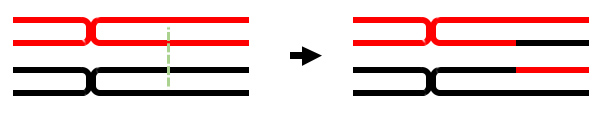
\includegraphics[width=0.7\textwidth]{../Figures/crossover1.jpg}%
	\vspace{-0.3cm}
	\captionof{figure}{Croisement en un point.}\label{croisement1}%
\end{center}



\paragraph{Deux points de croisement}
Pour deux points de croisement, chaque parent (solution) devra être fragmentée en trois, ainsi 
%TODO : solution parente ?
 chaque solution fils héritera de trois fragments (1 d'un parent et 2 de l'autre), comme représentés dans la figure \ref{croisement2} ci-dessous.
\begin{center}
	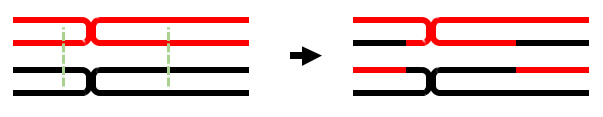
\includegraphics[width=0.7\textwidth]{../Figures/crossover2.jpg}%
	\vspace{-0.3cm}
	\captionof{figure}{Croisement en deux points.}\label{croisement2}%
\end{center}


\subsubsection{Opération de mutation}
La mutation apporte l'aléa nécessaire à une exploration efficace de l'espace des solutions en permettant de quitter les extrêmes locaux.
Il existe plusieurs façons de procéder à une mutation:


\paragraph{Inversement d'un gène}
Cette méthode consiste en l'inversement ou la troncature  d'un certain nombre fixe ou aléatoire de gènes d'une solution. La figure \ref{mut1} en est un exemple.
\begin{center}
	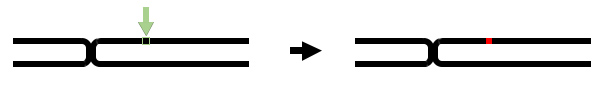
\includegraphics[width=0.7\textwidth]{../Figures/mutation1.jpg}%
	\vspace{-0.3cm}
	\captionof{figure}{Mutation avec inversement.}\label{mut1}%
\end{center}


\paragraph{Permutation de gènes}
Comme le montre la figure \ref{mut2}, 
la permutation de gènes nécessite d'abord la sélection de deux gènes sur l'individu (chromosome) à muter. Puis vient l'échange des deux valeurs (allèles) correspondantes, cela produit un nouvel individu. 
\begin{center}	
	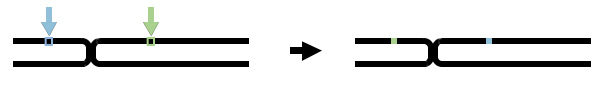
\includegraphics[width=0.7\textwidth]{../Figures/mutation2.jpg}%
	\vspace{-0.3cm}
	\captionof{figure}{Mutation avec permutation.}\label{mut2}%
\end{center}



\subsection{Pseudo code (GA incrémental)}
\begin{algorithm}[H]
	\TitleOfAlgo{GA}
	\vspace{-0.2cm}	
	\xdash[13.5cm]
	
	\SetAlgoLined
	\KwIn{$N$ : taille de la population, $MaxGen$ : nombre maximal de générations }
	\KwOut{meilleure solution}
	
	\SetKwFunction{GenerationSolutions}{GénérationSolutions}
	\SetKwFunction{Evaluation}{Evaluation}
	\SetKwFunction{MeilleurIndividus}{MeilleurIndividus}
	\SetKwFunction{PointCroisement}{PointCroisement}
	\SetKwFunction{Croisement}{Croisement}
	\SetKwFunction{NombreMutation}{NombreMutation}
	\SetKwFunction{Insertion}{Insertion}
	
	
	\Begin{
	$K \gets 0$\;
	$P_{k}\gets$ \GenerationSolutions(N)\;
	
	
	\Evaluation$(P_{k})$; \tcc{Évaluation de tous les individus de la population}
	
	\vspace{0.3cm}
	\While{$\neg$ $ BonneSolution$ \& $k < MaxGen$}{
		\tcc{Sélection des deux meilleurs parents de la population}
		$(Parent1 , Parent2)\gets$ \MeilleurIndividus$(P_{K})$\;
		
		\vspace{0.3cm}
		
		\tcc{Calcul da la position du point de croisement.}
		$i \gets$ \PointCroisement$(taille(solution))$\;
		\vspace{0.1cm}
		\tcc{Croisement des solutions parents}
		$Fils1 \gets$ \Croisement$(Parent1,Parent2,i)$\;
		$Fils2 \gets$ \Croisement$(Parent2,Parent1,i)$\;
		\vspace{0.1cm}
		\tcc{Évaluation des solutions fils}
		\Evaluation($Fils1$); 
		\Evaluation($Fils2$)\;
		
		\vspace{0.3cm}
		
		\tcc{Détermination du nombre de mutations.}
		$j \gets$ \NombreMutation$(taille(solution))$\;
		\vspace{0.1cm}
		\tcc{Mutation des solutions fils}
		$FilsMutant1 \gets Mutation(Fils1,j)$\;
		$FilsMutant2 \gets Mutation(Fils2,j)$\;
		\vspace{0.1cm}
		\tcc{Évaluation des solutions fils mutantes}
		\Evaluation($FilsMutant1$); \Evaluation($FilsMutant2$)\;
		
		
		\vspace{0.3cm}
		
		$K \gets K +1$\;
		\vspace{0.1cm}
		\tcc{Mise à jour de la population, suppression des solutions parents et insertion des solutions fils et fils mutantes.}
		$K \gets K +1$; 
		\Insertion$(P_{k},Newindividus)$\;	
	}
}
	
	\caption{Algorithme Génétique}
\end{algorithm}


\section{Conclusion}
Comme on a pu le constater, le comportement collectif des éléphants et des abeilles ainsi que la complexité de leur psychologie ont donné lieu à de puissants algorithmes de résolution orientés espaces des solutions. Ces derniers ont prouvé leur performance et leur efficacité face à de nombreux problèmes.
Ainsi, vu notre problématique, qui rappelons-le, consiste à détecter des cibles dans un espace complexe inconnu à l'aide de robots mobiles, nous avons choisi ces algorithmes intelligents pour la
résolution de notre problème compte tenu de leur robustesse. Le chapitre qui suit portera sur la modélisation de notre solution sur laquelle se baseront nos différentes approches mono-BSO, multi-BSO, EHO ainsi qu'ESWSA.



